\begin{pagefigure}
\centering
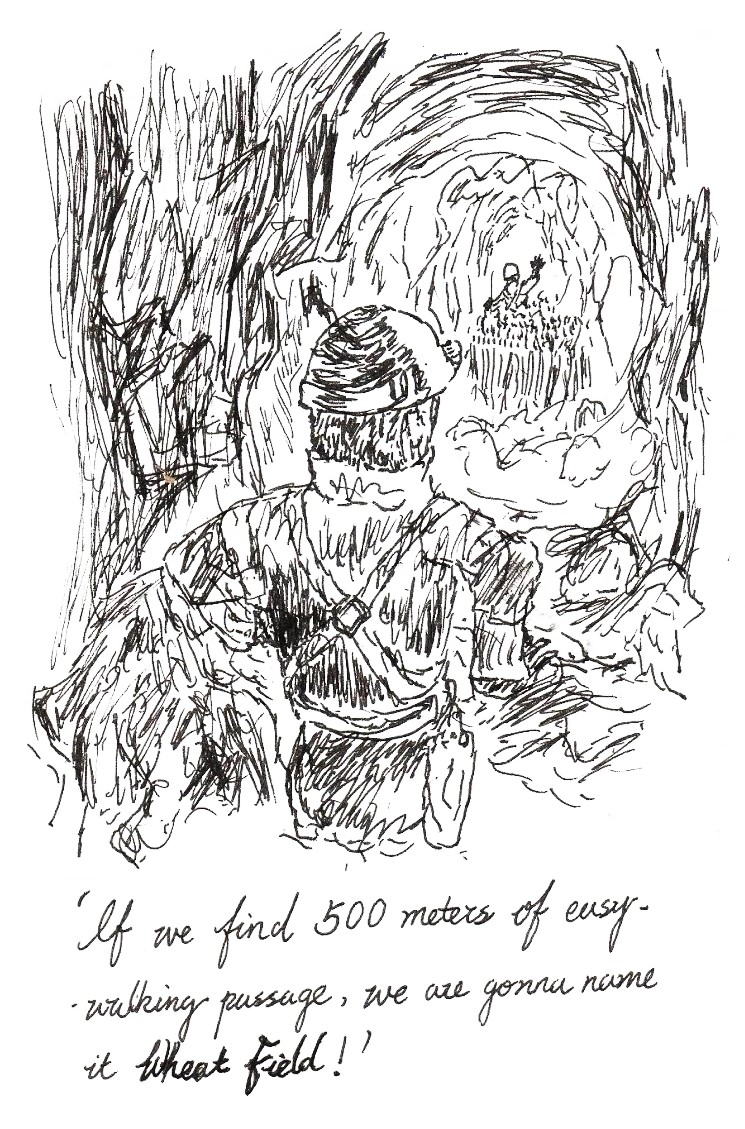
\includegraphics[width=0.9\linewidth]{images/overview/the_caver_2.jpg}
\caption{Drawn by Larry Jiyu Jiang}
\label{}
\end{pagefigure}
\newpage


\begin{tcolorbox} %makes a white opaque background for the text.
\vspace{60pt}
	\part{Introduction}
	\lettrine{S}{istem} \passage{Migovec}, tucked away at the western edge of the \passage{Trigavski Narodni Park} is the longest cave system in Slovenia. It has been since 2012, when, defying the expectations after a half a decade of effort, the connection between the `\passage{Old System}' (\passage{M2}-\passage{M16}-\passage{M18}) and the newer \passage{Vrtnarija} (\passage{Gardeners' World}) and \passage{Vilinska Jama} cave was forged after a routine pushing trip at -600m. This - 38 years since the beginnings of exploration underneath \passage{Tolminski Migovec}, `\passage{Mig}' as it is affectionately named - made the national news. 

Since then, and rather more discreetly,  Imperial College cavers (ICCC) have repeatedly spent their summers discovering more voids under the hollow mountain, in tandem with the Jamarska Sekcija Planinskega Drustva Tolmin (hereafter JSPDT). Bit by bit, the other pieces of the puzzle were extended and connected to the main system. In October 2015, three Slovene cavers found a way between the last big independent cave system, \passage{Primadona}-\passage{Monatip}-\passage{Ubend571} and one of the earliest high level passages of \passage{Sistem Migovec}, bringing the total to 35.6km of connected passage. Since October 2017, it stands at 39.2km.

This book is divided in three parts. The introduction to the geography and geology of \passage{Tolminski Migovec}, the process of cave exploration and survey aims to give a cursory glance at the setting and logistics of the expeditions. This is followed by the main body of text: selected stories from expedition cavers, by no means a complete account of all the excursions under the mountain. These span the years 2013-2017, which saw systematic summer expeditions by ICCC and continuous JSPDT action. A third part provides a more detailed description of possible trips within the mountain, augmented with larger scale surveys: they are intended for expedition cavers craving to see more of this nearly 40km alpine system. 
\end{tcolorbox}
	\backgroundsetup{	scale=1,
					color=black,
					opacity=1,
					angle=0,
					contents={%
							  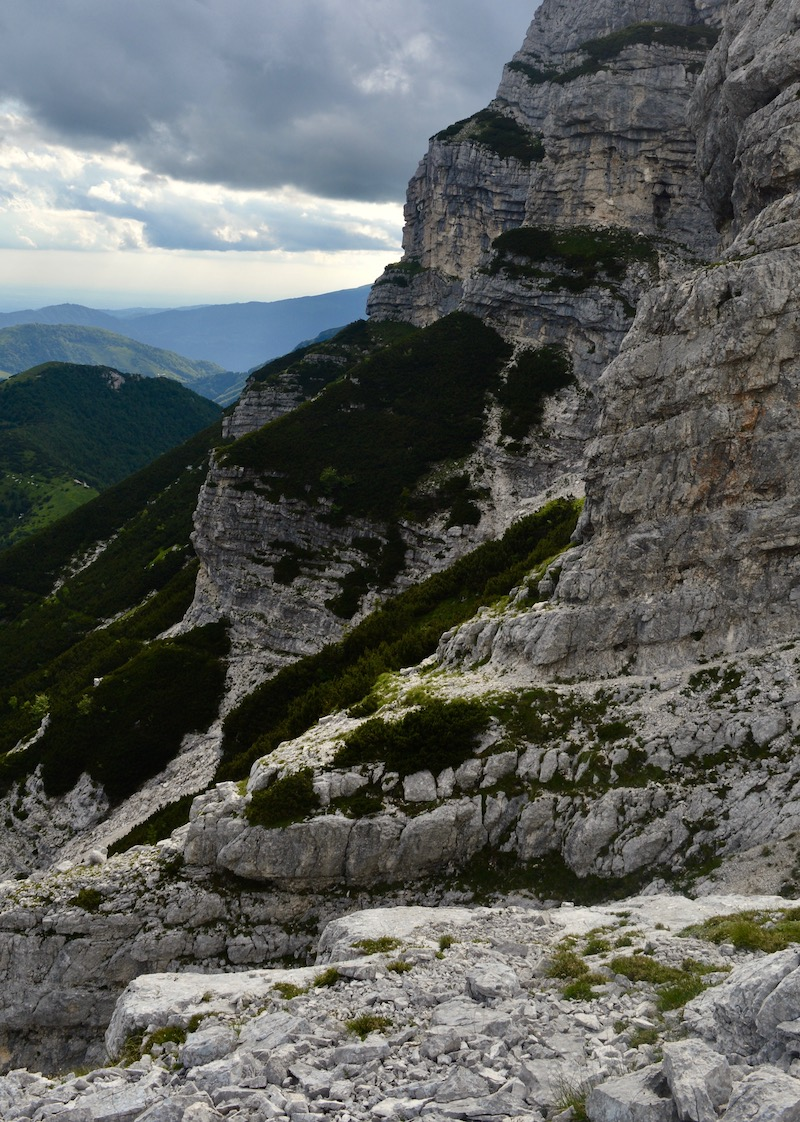
\includegraphics[height=\paperheight]{images/backgrounds/migface.jpg}
  					} % this puts the entire image as local background
	}
\BgThispage %calls the image to be displayed as background, flush with paper edge.
